\documentclass{../source/Experiment}

\major{信息工程}
\name{姚桂涛}
\title{喇叭天线的幅射特性测量及CST仿真}
\stuid{3190105597}
\college{信息与电子工程学院}
\date{\today}
\lab{东4-221}
\course{电磁场与电磁波}
\instructor{王子立}
\grades{}
\expname{喇叭天线的幅射特性测量及CST仿真}
\exptype{}
\partner{}

\usepackage{caption}

\DeclareCaptionLabelSeparator{twospace}{\, }
\captionsetup{labelsep = twospace}

\begin{document}
    \makecover
    \makeheader

    \begin{center}
        \bfseries\Large{矩形波导馈电的角锥喇叭天线CST仿真}
    \end{center}
    \section{实验目的}
        \begin{enumerate}
            \item 了解并掌握波导喇叭天线的常用参数指标和分析方法.
            \item 了解熟悉CST软件的基本使用方法,学会运用其进行建模、仿真。
        \end{enumerate}
    \section{实验任务}
        用CST软件对特定的巨型波导喇叭天线进行建模、仿真,分析其辐射特性,并与喇叭天线辐射特性测量实验进行比较。
    \section{实验过程与结果}
        \subsection{模型建立}
            \subsubsection{建立工程}
                \begin{figure}[H]
                    \centering
                    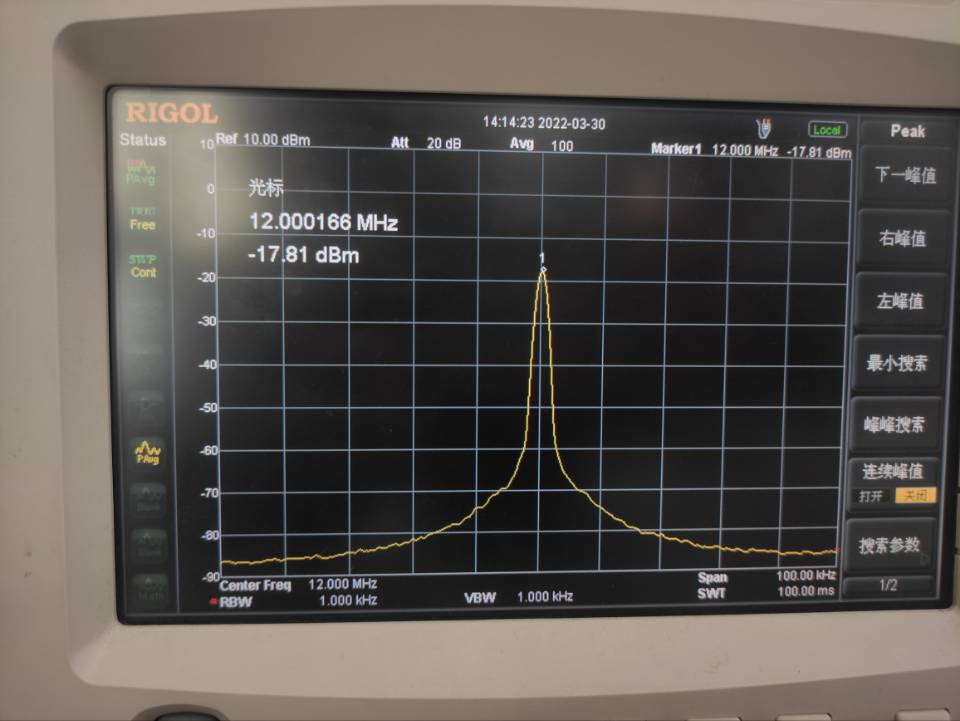
\includegraphics[width = 0.6\textwidth]{1}
                    \caption{}
                \end{figure}

                \begin{figure}[H]
                    \centering
                    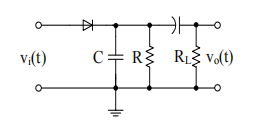
\includegraphics[width = 0.6\textwidth]{2}
                    \caption{}
                \end{figure}

            \subsubsection{参数设置}
                \begin{figure}[H]
                    \centering
                    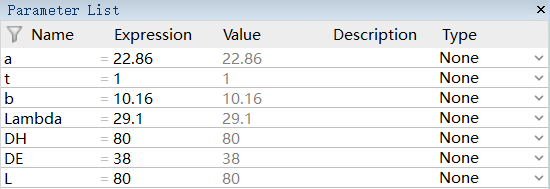
\includegraphics[width = 0.6\textwidth]{0}
                    \caption{}
                \end{figure}
            \subsubsection{创建矩形}

            \begin{figure}[H]
                \centering
                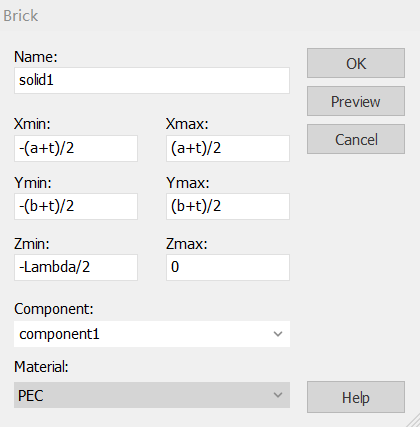
\includegraphics[width = 0.5\textwidth]{3}
                \caption{}
            \end{figure}
            
            \begin{figure}[H]
                \centering
                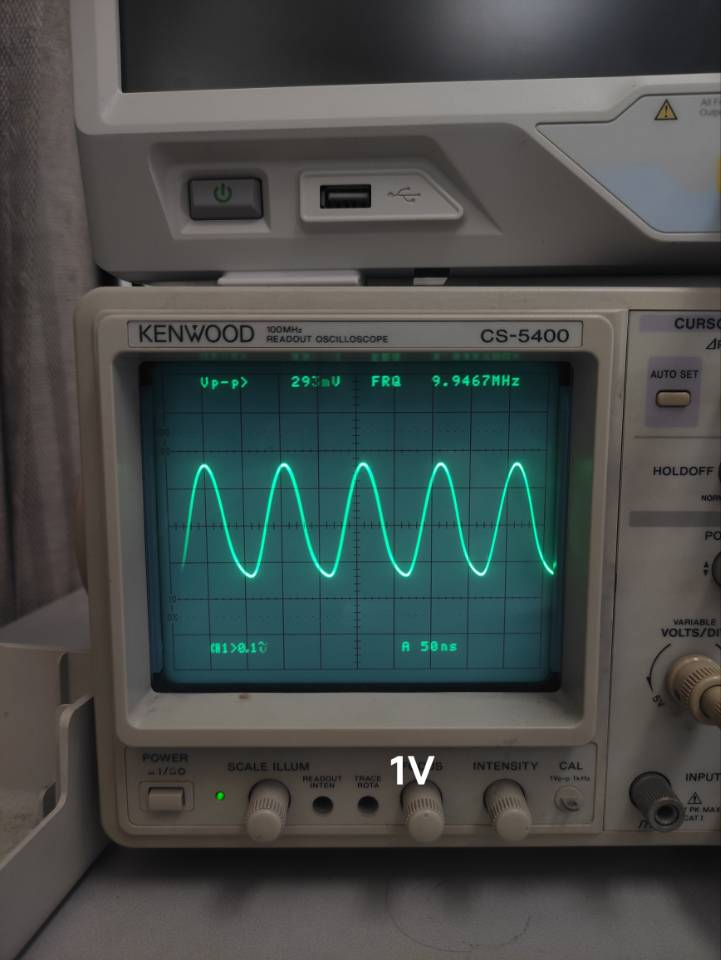
\includegraphics[width = 0.8\textwidth]{4}
                \caption{}
            \end{figure}
            
            \subsubsection{建立喇叭模型}

            建立喇叭口径面
            \begin{figure}[H]
                \centering
                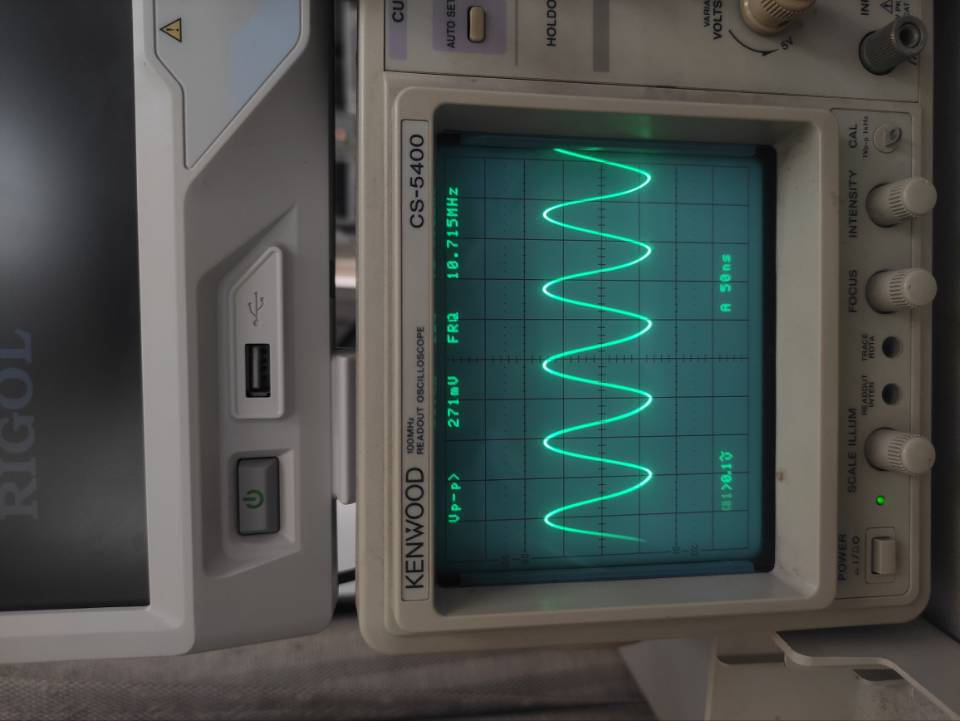
\includegraphics[width = 0.4\textwidth]{5}
                \caption{}
            \end{figure}

            \begin{figure}[H]
                \centering
                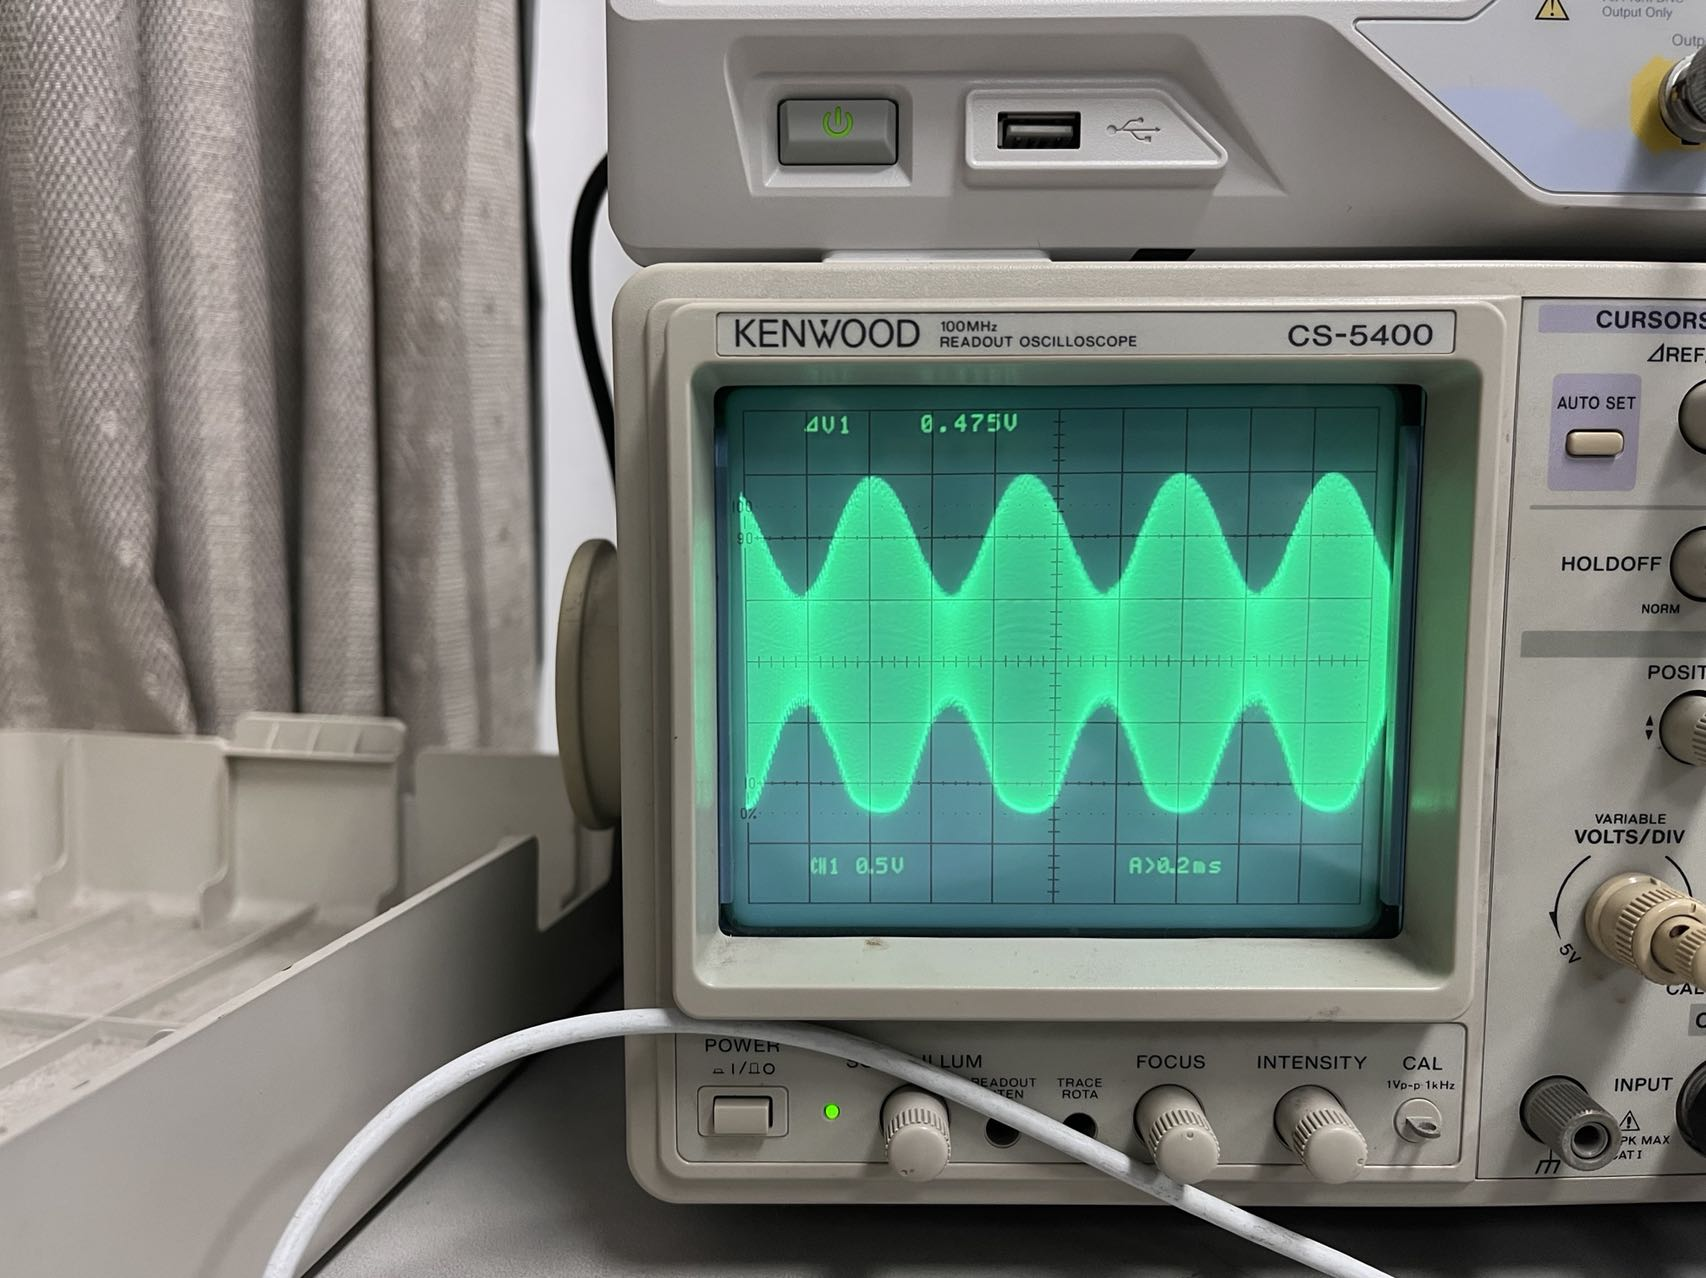
\includegraphics[width = 0.4\textwidth]{7}
                \caption{}
            \end{figure}

            \begin{figure}[H]
                \centering
                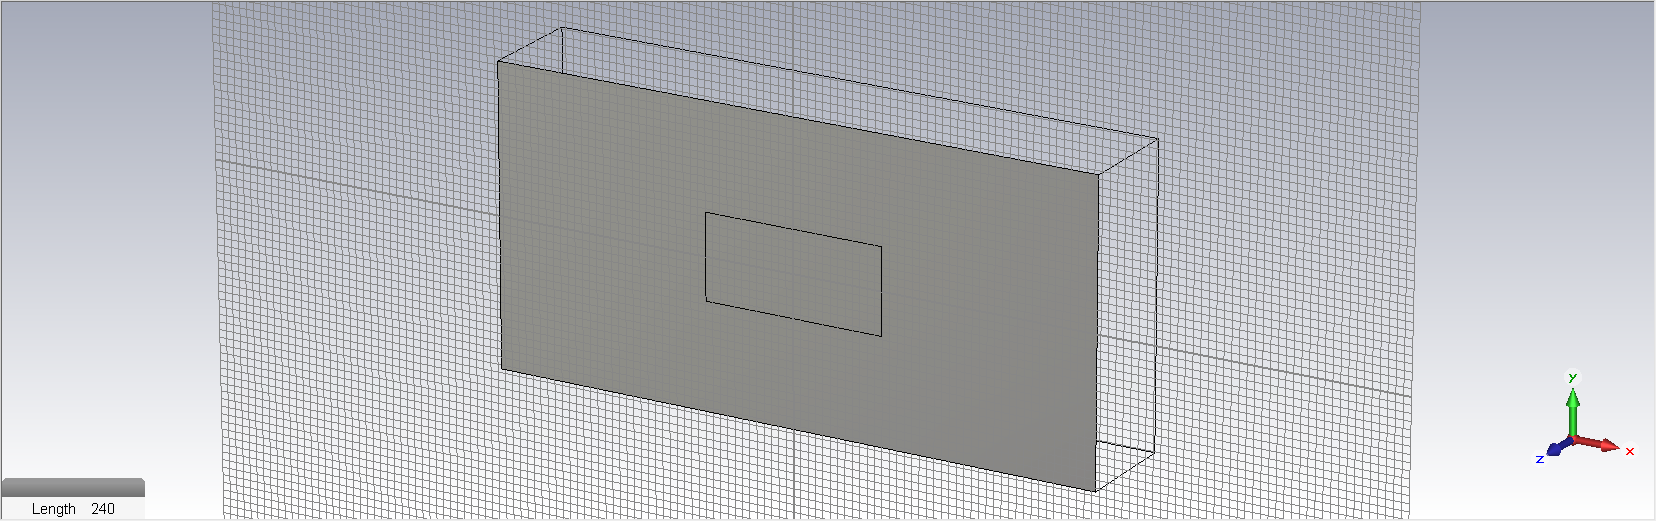
\includegraphics[width = 0.8\textwidth]{8}
                \caption{}
            \end{figure}


            设置喇叭口径面的空间位置

            \begin{figure}[H]
                \centering
                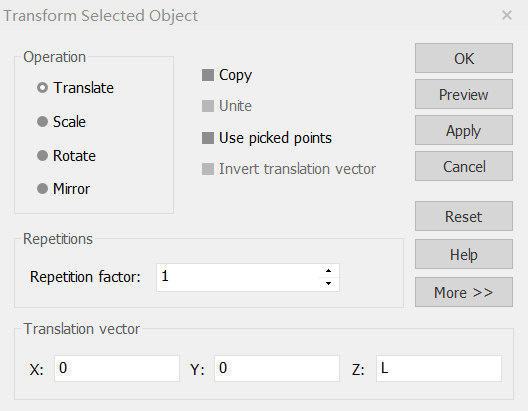
\includegraphics[width = 0.6\textwidth]{9}
                \caption{}
            \end{figure}


            \begin{figure}[H]
                \centering
                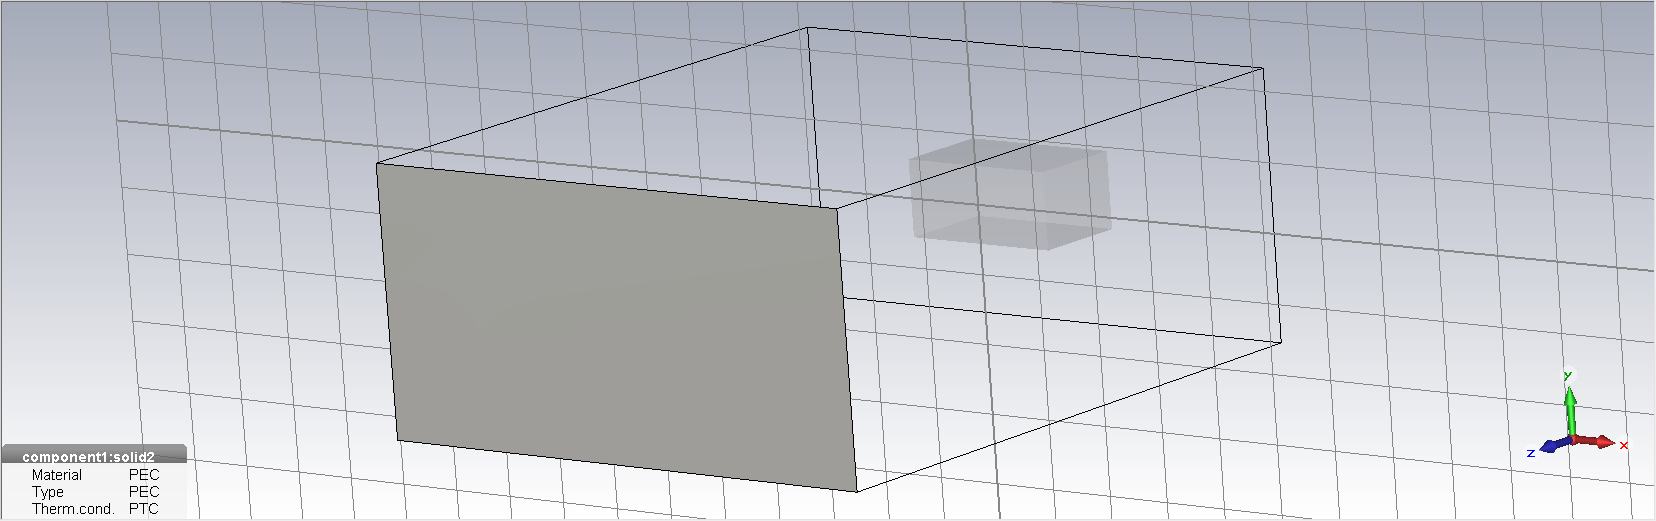
\includegraphics[width = 0.8\textwidth]{10}
                \caption{}
            \end{figure}
            创建喇叭侧壁
            \begin{figure}[H]
                \centering
                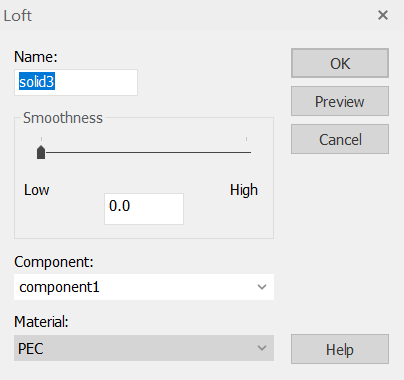
\includegraphics[width = 0.4\textwidth]{11}
                \caption{}
            \end{figure}
            \begin{figure}[H]
                \centering
                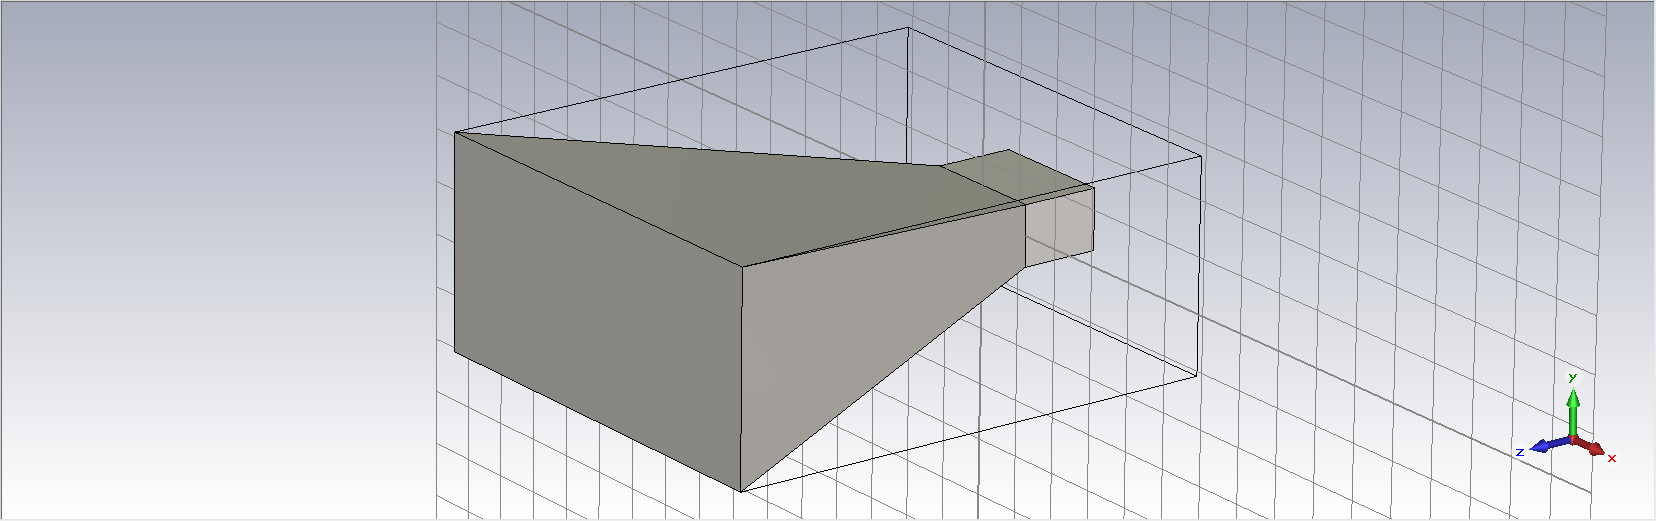
\includegraphics[width = 0.8\textwidth]{12}
                \caption{}
            \end{figure}

            掏空
            \begin{figure}[H]
                \centering
                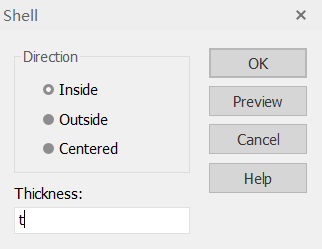
\includegraphics[width = 0.4\textwidth]{13}
                \caption{}
            \end{figure}
            \begin{figure}[H]
                \centering
                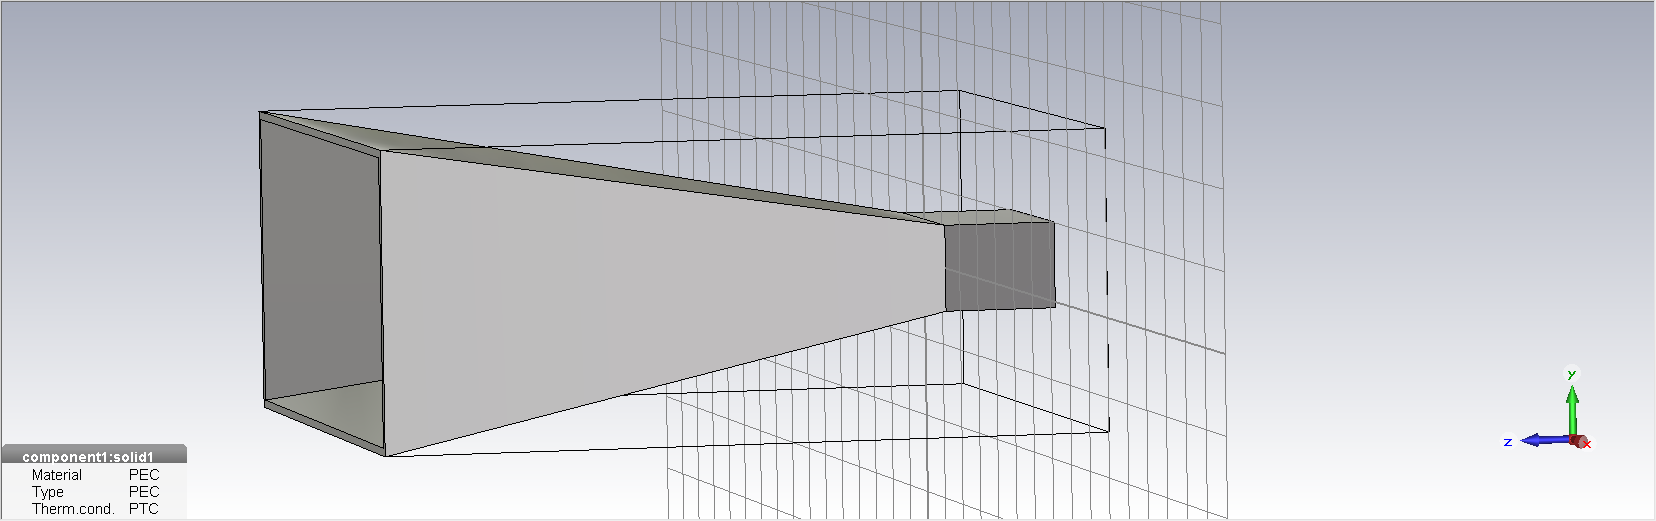
\includegraphics[width = 0.8\textwidth]{14}
                \caption{}
            \end{figure}

        \subsection{仿真分析}

            \subsubsection{仿真条件设置}
            仿真频率
            \begin{figure}[H]
                \centering
                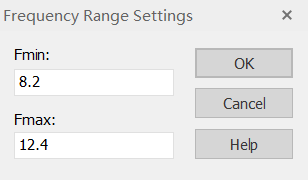
\includegraphics[width = 0.3\textwidth]{15}
                \caption{}
            \end{figure}
            仿真边界条件
            \begin{figure}[H]
                \centering
                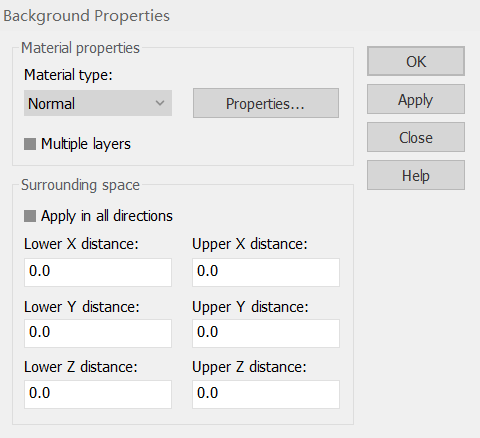
\includegraphics[width = 0.6\textwidth]{16}
                \caption{}
            \end{figure}
            
            \begin{figure}[H]
                \centering
                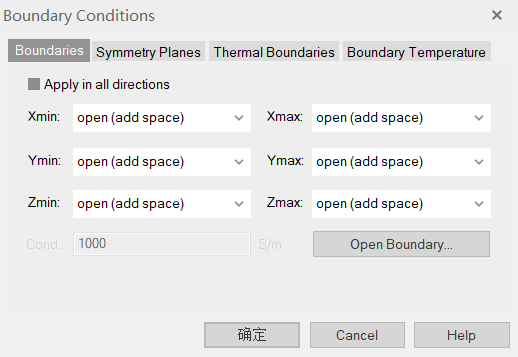
\includegraphics[width = 0.6\textwidth]{17}
                \caption{}
            \end{figure}

            端口设置
            \begin{figure}[H]
                \centering
                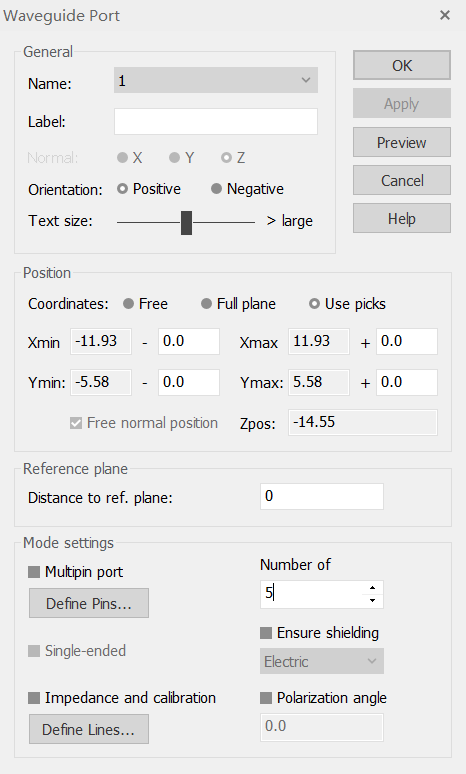
\includegraphics[width = 0.6\textwidth]{18}
                \caption{}
            \end{figure}
            设置监视器
            
            \begin{figure}[H]
                \centering
                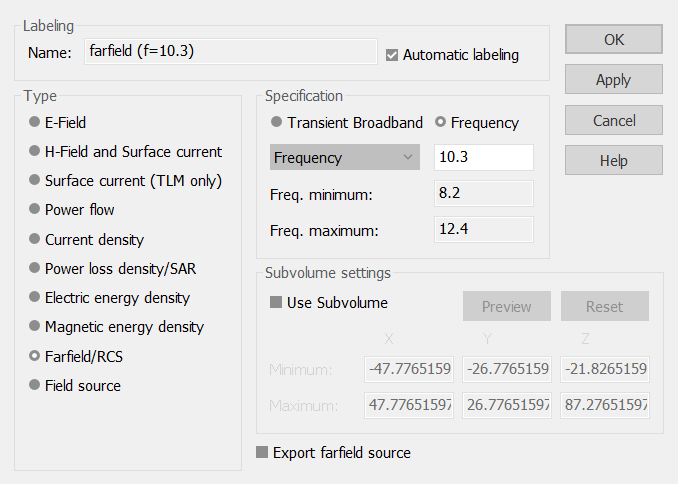
\includegraphics[width = 0.7\textwidth]{20}
                \caption{}
            \end{figure}
            \begin{figure}[H]
                \centering
                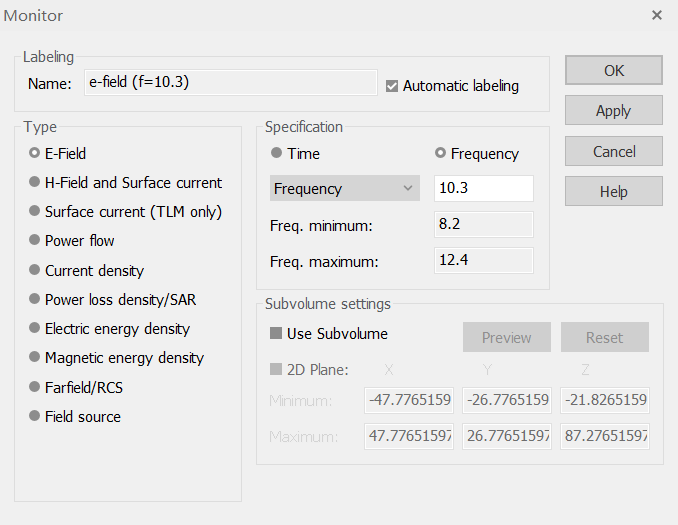
\includegraphics[width = 0.7\textwidth]{24}
                \caption{}
            \end{figure}
            \begin{figure}[H]
                \centering
                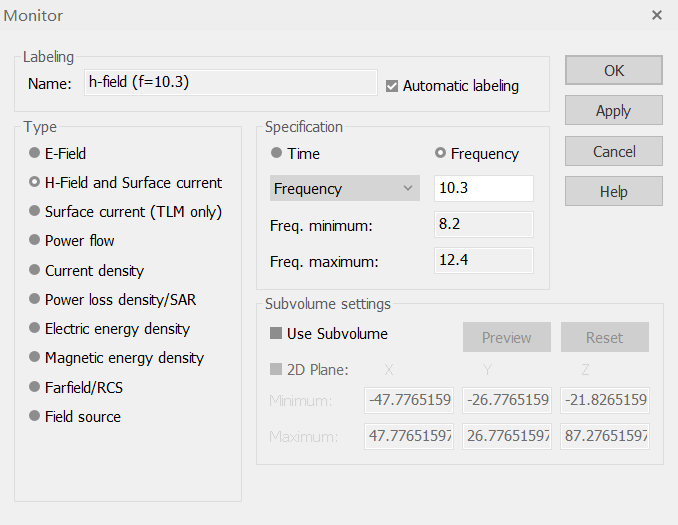
\includegraphics[width = 0.7\textwidth]{25}
                \caption{}
            \end{figure}
            
            \subsubsection{模式分析}
            \begin{figure}[H]
                \centering
                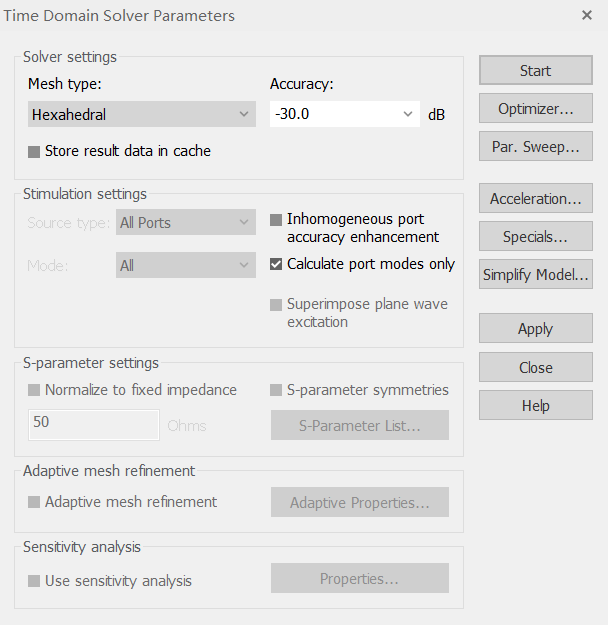
\includegraphics[width = 0.7\textwidth]{21}
                \caption{}
            \end{figure}
            \begin{figure}[H]
                \centering
                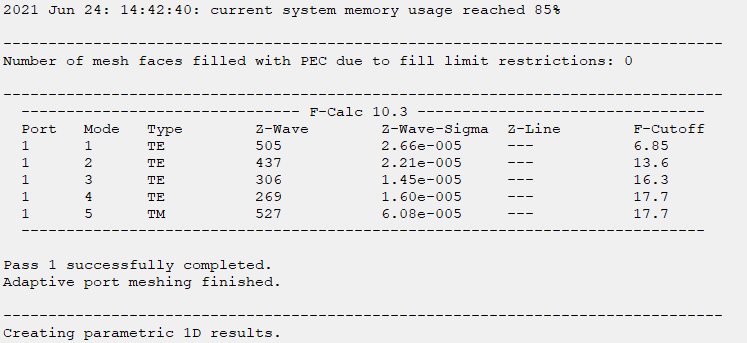
\includegraphics[width = 0.7\textwidth]{22}
                \caption{}
            \end{figure}
            

            由于仿真最高频率为12.4GHz,所以在这种结构的喇叭天线中只传输1 种模式的波,设置的吸收的模式数只要大于1 就可以了。
            \subsubsection{仿真设置}
            \begin{figure}[H]
                \centering
                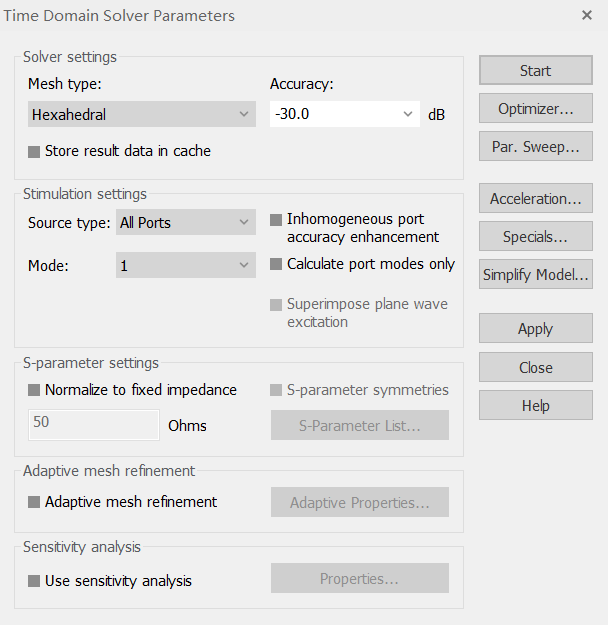
\includegraphics[width = 0.7\textwidth]{23}
                \caption{}
            \end{figure}
            
        \subsection{仿真结果}

            \subsubsection{$S_{11}$曲线}
            \begin{figure}[H]
                \centering
                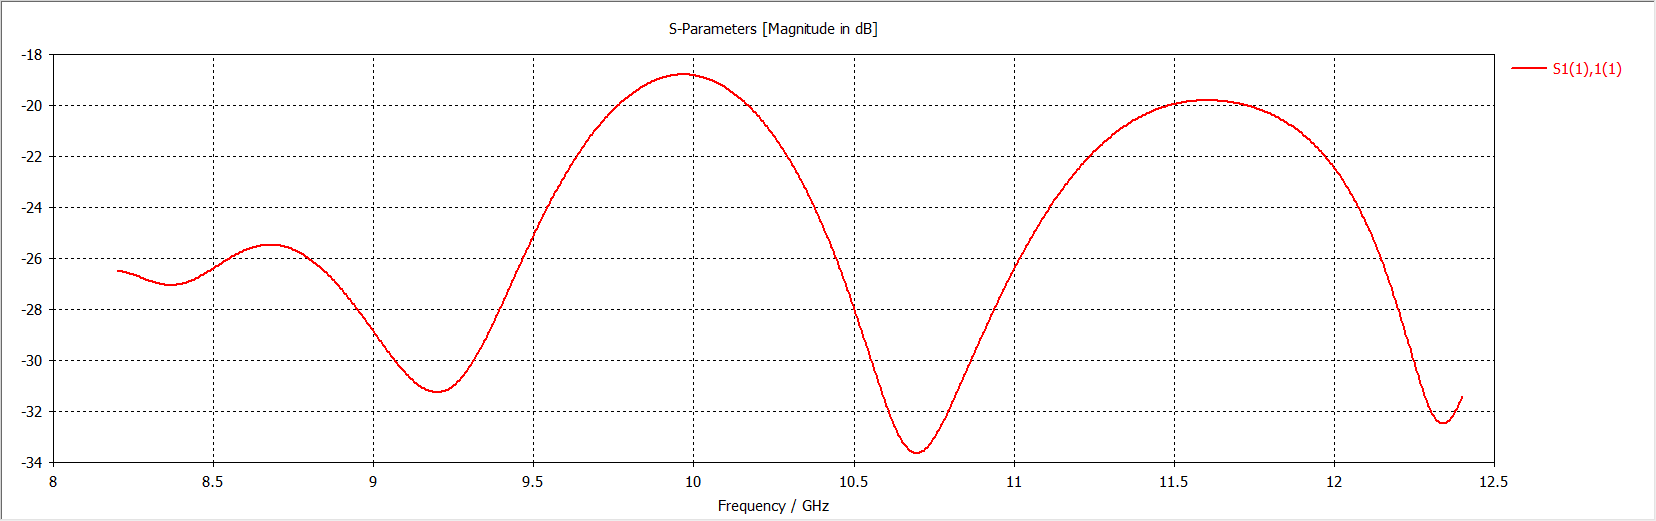
\includegraphics[width = 0.8\textwidth]{S11}
                \caption{}
            \end{figure}
            
            \subsubsection{驻波曲线}
            \begin{figure}[H]
                \centering
                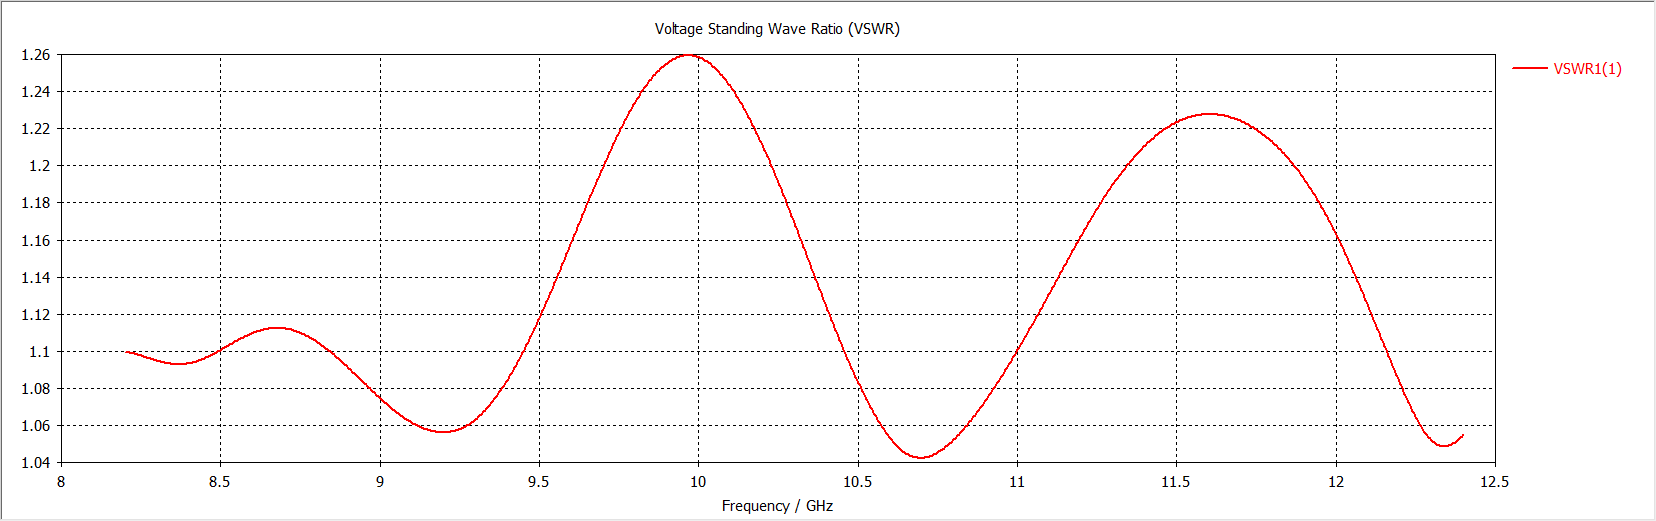
\includegraphics[width = 0.8\textwidth]{VSWR}
                \caption{}
            \end{figure}
            
            \subsubsection{方向图}
            \begin{figure}[H]
                \centering
                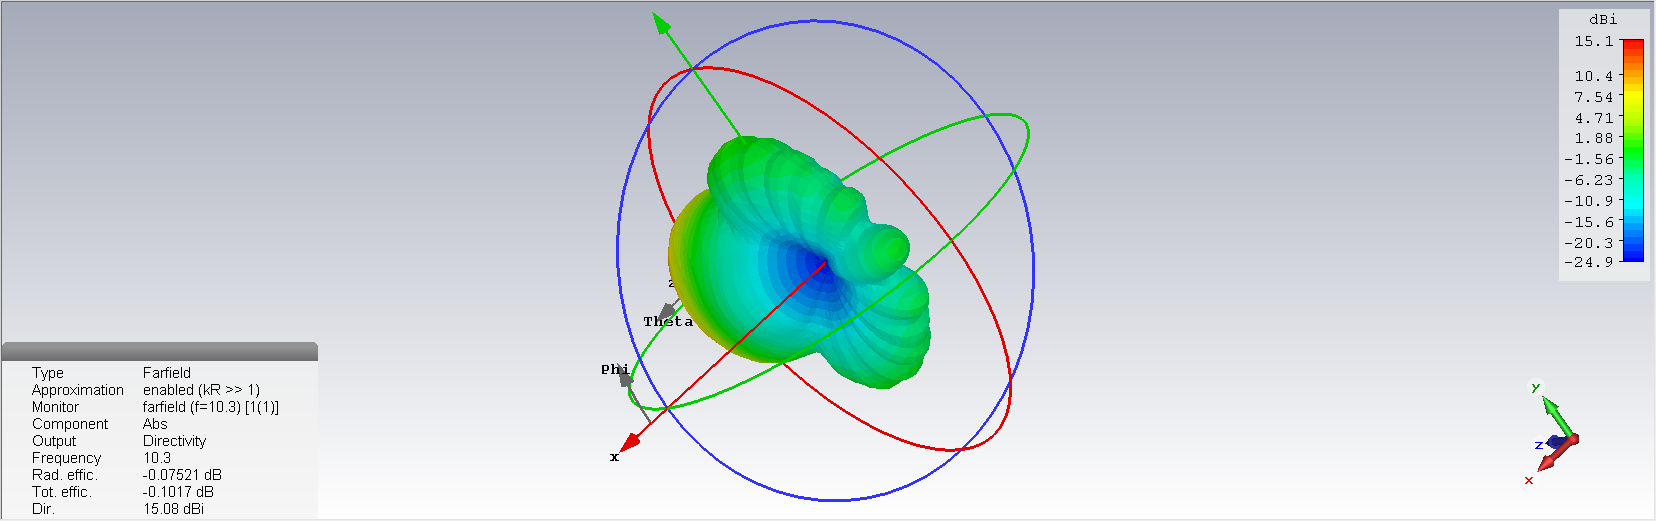
\includegraphics[width = 0.8\textwidth]{Directivity}
                \caption{}
            \end{figure}
            \begin{figure}[H]
                \centering
                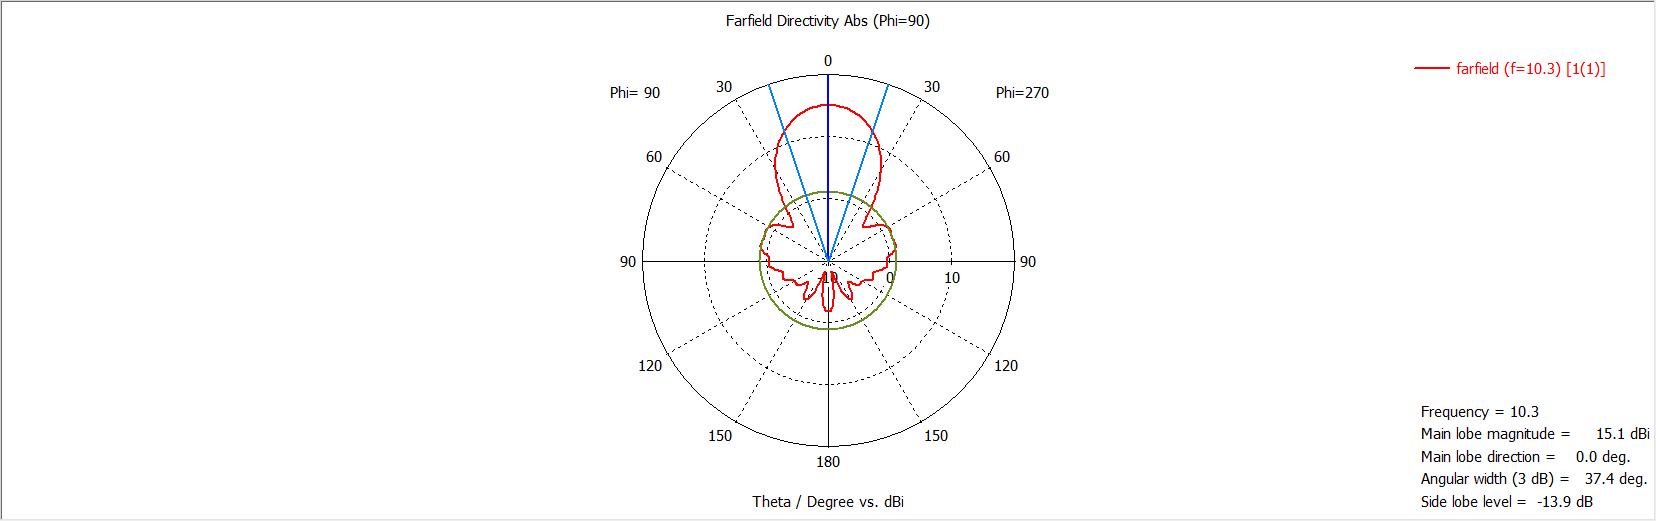
\includegraphics[width = 0.8\textwidth]{Directivity Polar}
                \caption{}
            \end{figure}
            
            \subsubsection{增益图}
            \begin{figure}[H]
                \centering
                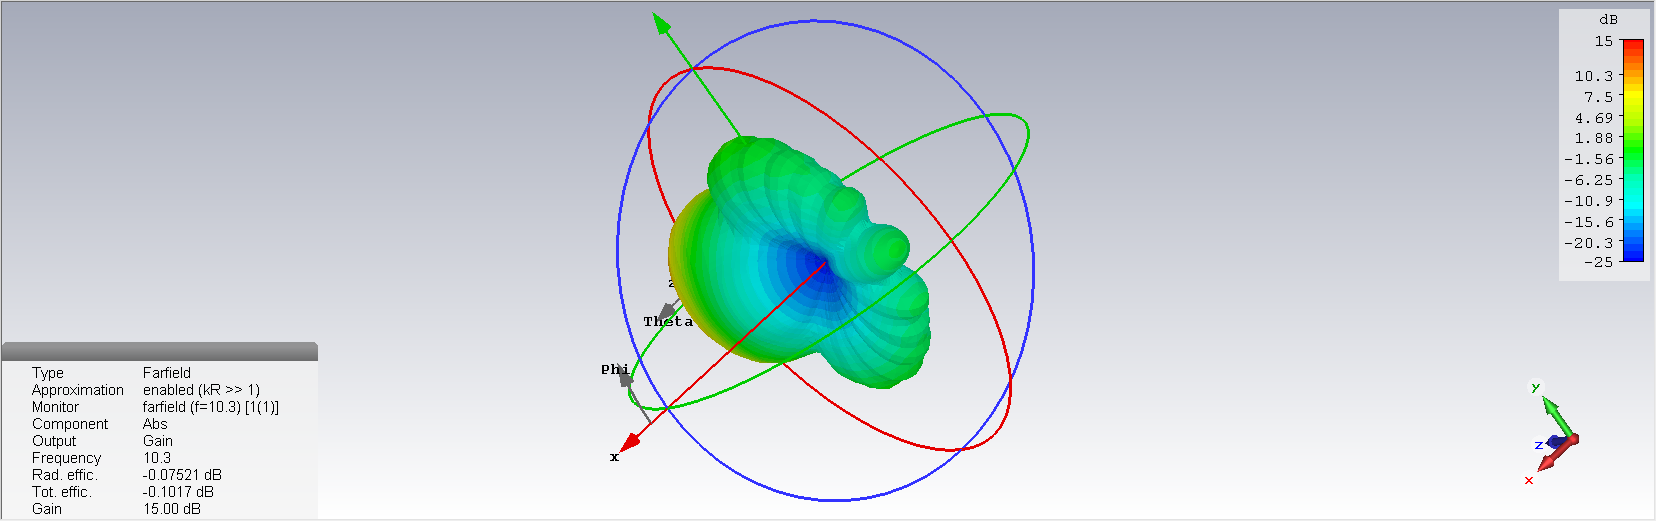
\includegraphics[width = 0.8\textwidth]{Gain}
                \caption{}
            \end{figure}
            \begin{figure}[H]
                \centering
                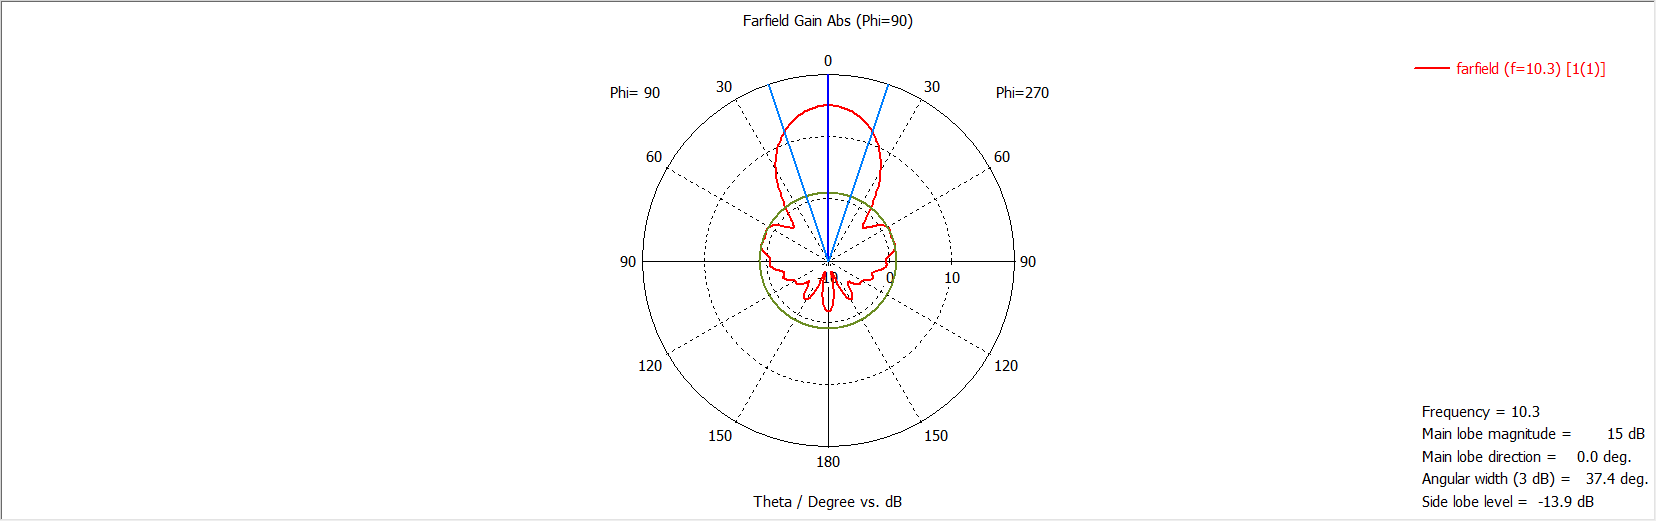
\includegraphics[width = 0.8\textwidth]{Gain polar}
                \caption{}
            \end{figure}
            
            \subsubsection{E-field,  H-field,  surface current图}
            \begin{figure}[H]
                \centering
                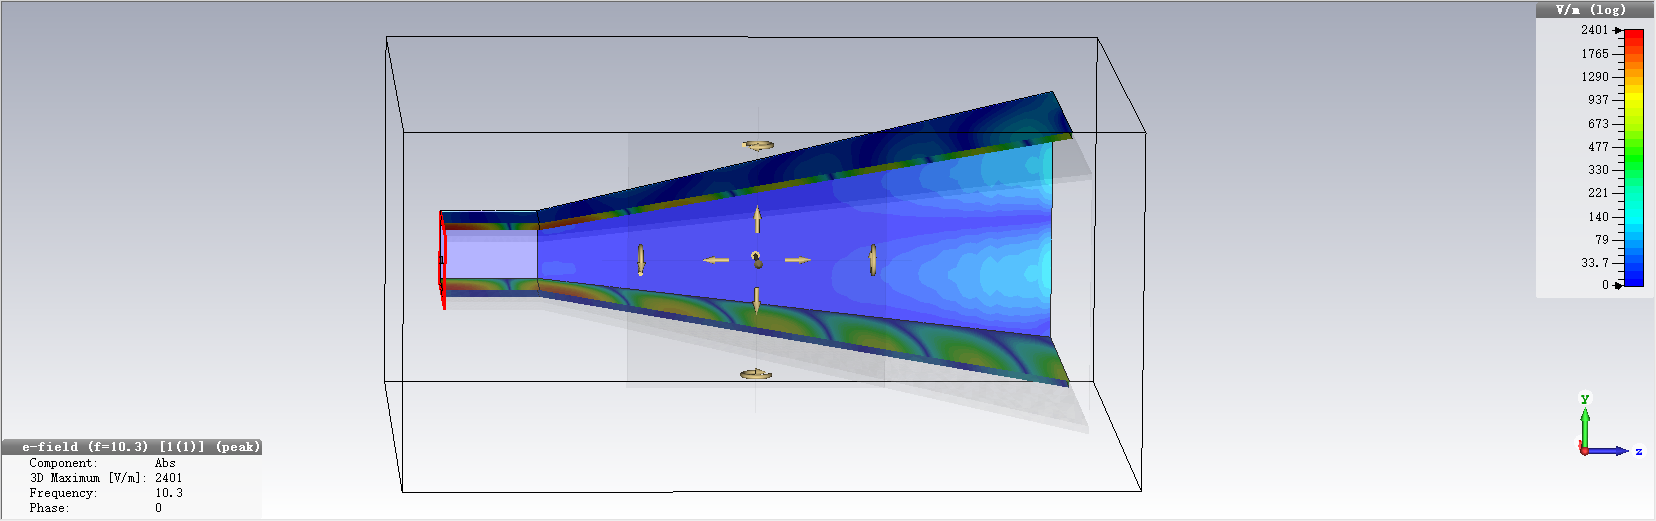
\includegraphics[width = 0.8\textwidth]{e-field}
                \caption{e-field}
            \end{figure}
            \begin{figure}[H]
                \centering
                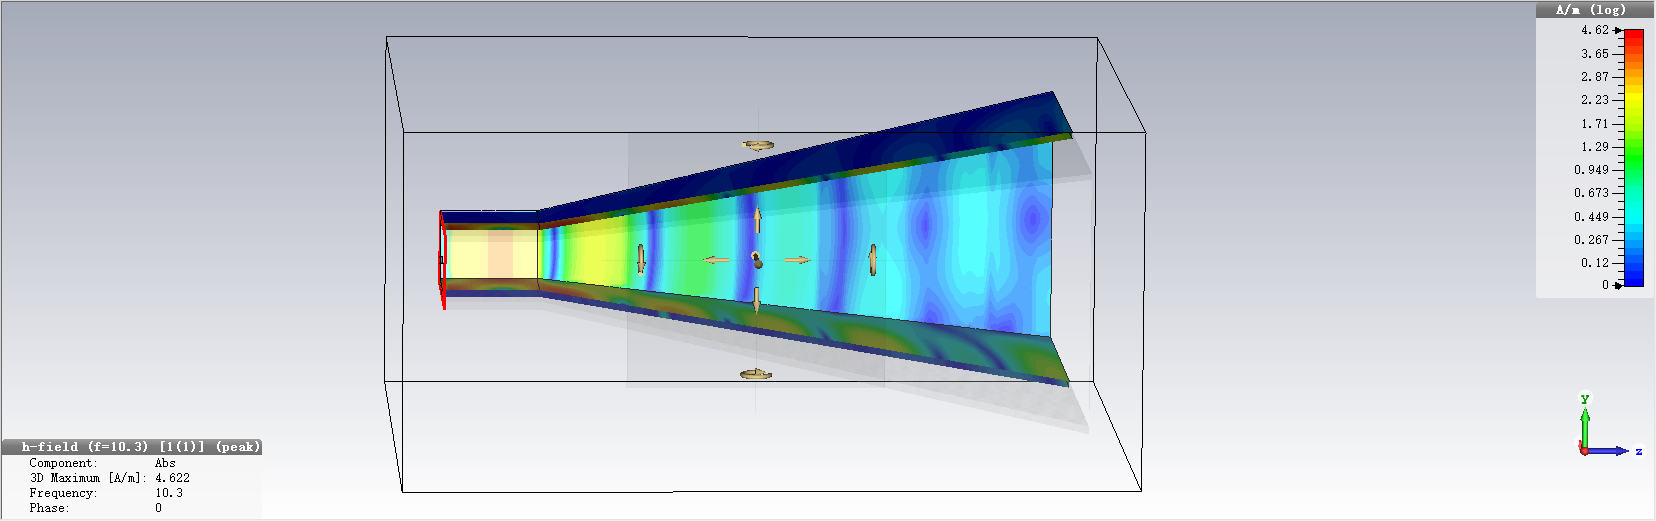
\includegraphics[width = 0.8\textwidth]{h-field}
                \caption{h-field}
            \end{figure}
            \begin{figure}[H]
                \centering
                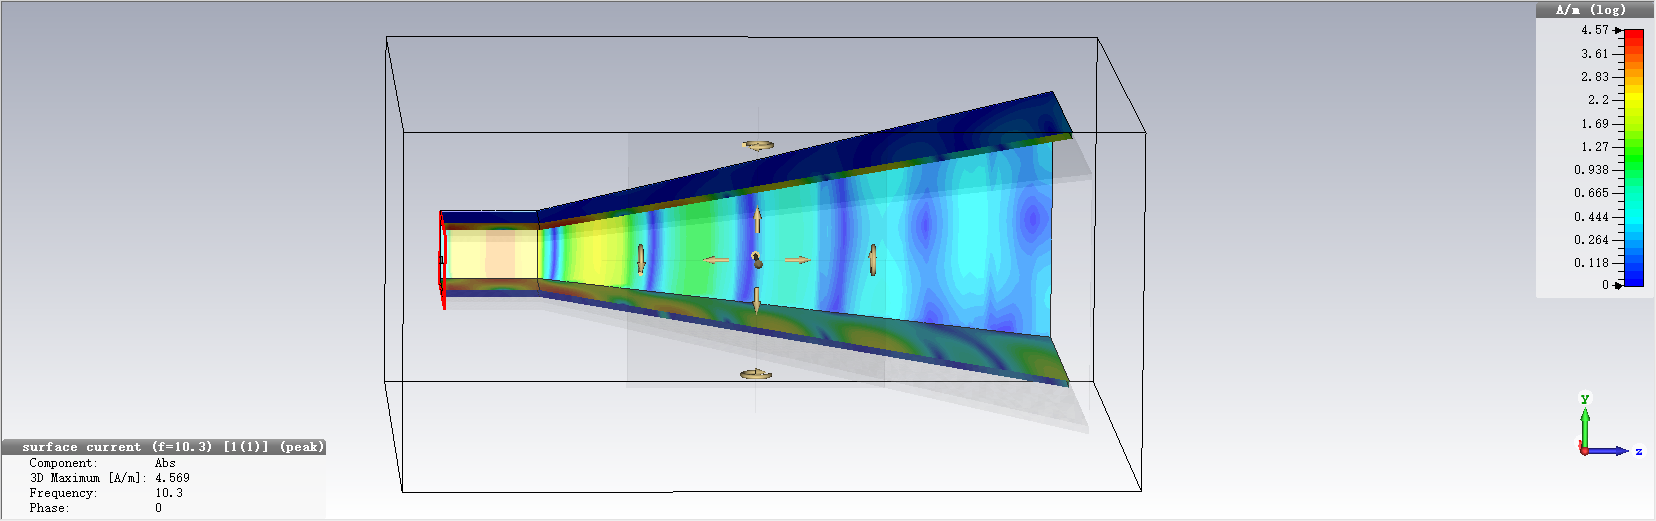
\includegraphics[width = 0.8\textwidth]{surface}
                \caption{surface current}
            \end{figure}
            
        \subsection{分析结论}

            从仿真结果来看,该矩形波导馈电的角锥喇叭天线的主瓣方向为$ \varphi = 0 \deg ,\, \theta = 0 \deg$,主瓣宽度为37.4\degree ,主瓣的最大增益为15dB,最大增益的仿真值与
            理论估计值相近。同时,该天线输入端口的反射系数在工作频段内均在20dB 以下,能够较好的工作。

    \section{实验收获与体会}

    \setcounter{section}{0}

    \begin{center}
        \bfseries\Large{喇叭天线的幅射特性测量}
    \end{center}

    \section{实验目的}
        揭示喇叭天线的幅射特性。 \par 
        覆盖的基本概念:
        \begin{itemize}
            \item 天线辐射方向图
            \item 波束宽度
            \item 天线的极化特性
            \item 电磁波在空间传播中与距离的关系
        \end{itemize}
    \section{实验过程与结果}
        \subsection{电磁波在空间传播中与距离的关系测量}
            \begin{table}[H]
                \caption{天线距离与接收功率关系}
                \centering
                \begin{tabular}{|c|c|c|}
                \hline
                距离R(m) & 实验测量值(dB) & 相对归一化功率(dB) \\ \hline
                1.0    & -40.0     & 0.0         \\ \hline
                1.1    & -41.8     & -1.8        \\ \hline
                1.2    & -43.6     & -3.6        \\ \hline
                1.3    & -45.3     & -5.3        \\ \hline
                1.4    & -46.8     & -6.8        \\ \hline
                \end{tabular}
            \end{table}
        \subsection{极化测量}
            \subsubsection{天线极化测量}
                \begin{table}[H]
                    \caption{发射喇叭天线极化特性}
                    \centering
                    \begin{tabular}{|c|c|c|}
                    \hline
                    发射喇叭天线角度                 & 实验测量值(dB) & 相对归一化功率(dB) \\ \hline
                    0\degree  & -40.0     & 0.0         \\ \hline
                    10\degree & -47.0     & -7.0        \\ \hline
                    20\degree & -55.6     & -15.6       \\ \hline
                    30\degree & -61.6     & -21.6       \\ \hline
                    40\degree & -63.6     & -23.6       \\ \hline
                    50\degree & -68.4     & -28.4       \\ \hline
                    60\degree & -71.0     & -31.0       \\ \hline
                    70\degree & -76.0     & -36.0       \\ \hline
                    80\degree & -80.0     & -40.0       \\ \hline
                    90\degree & -80.0     & -40.0       \\ \hline
                    \end{tabular}
                \end{table}
            \subsubsection{极化栅网特性测量}
                \begin{table}[H]
                    \caption{极化栅网极化特性}
                    \centering
                    \begin{tabular}{|c|c|c|}
                    \hline
                    极化栅网角度                   & 实验测量值(dB) & 相对归一化功率(dB) \\ \hline
                    0\degree  & -40.0     & 0.0         \\ \hline
                    90\degree & -69.3     & -29.3       \\ \hline
                    45\degree & -44.5     & -4.5        \\ \hline
                    \end{tabular}
                \end{table}
        \subsection{喇叭天线辐射方向图测量}
        \begin{table}[H]
            \caption{天线水平方向图测量数据}
            \centering
            \resizebox{\textwidth}{!}{
            \begin{tabular}{|c|c|c|c|c|c|c|c|c|c|c|c|c|c|c|c|c|c|c|c|}
            \hline
            天线水平方向转角(\degree) & -90      & -80      & -70   & -60   & -50   & -40   & -30   & -20   & -10   & 0     & 10    & 20    & 30    & 40    & 50    & 60    & 70    & 80    & 90       \\ \hline
            实验测量值(dB)                        & $\infty$ & $\infty$ & -80.0 & -73.8 & -74.0 & -66.8 & -57.8 & -49.8 & -43.0 & -40.0 & -44.2 & -52.6 & -61.0 & -63.4 & -66.8 & -70.5 & -77.5 & -80.0 & $\infty$ \\ \hline
            相对归一化功率                          & $\infty$ & $\infty$ & -40.0 & -33.8 & -34.0 & -26.8 & -17.8 & -9.8  & -3.0  & 0.0   & -4.2  & -12.6 & -21.0 & -23.4 & -26.8 & -30.5 & -37.5 & -40.0 & $\infty$ \\ \hline
            \end{tabular}}
            \end{table}

            \begin{table}[H]
                \caption{天线垂直方向测量数据}
                \centering
                \resizebox{\textwidth}{!}{
                \begin{tabular}{|c|c|c|c|c|c|c|c|c|c|c|c|c|c|}
                \hline
                天线垂直方向转角(\degree) & -60   & -50   & -40   & -30   & -20   & -10   & 0     & 10    & 20    & 30    & 40    & 50    & 60    \\
                \hline
                实验测量值(dB)                        & -68.6 & -66.2 & -65.5 & -65.2 & -58.6 & -51.5 & -50.0 & -51.5 & -57.2 & -65.0 & -66.0 & -66.2 & -69.0 \\
                \hline
                相对归一化功率(dB)                      & -18.6 & -16.2 & -15.5 & -15.2 & -8.6  & -1.5  & 0.0   & -1.5  & -7.2  & -15.0 & -16.0 & -16.2 & -19.0 \\
                \hline
                \end{tabular}}
                \end{table}
    \section{思考题}

    \section{实验收获与体会}
\end{document}